\chapter{Future Work: Routing}

Once the placement phase is performed with the slicing tree, it is then used for the routing phase. For our analog routing approach, we will divide this step into two phases: a global routing phase and a detailed routing phase. To be able to route mixed-signal circuit, it is required to build a router capable of handling both digital and analog routing constraints. At the moment, our router can handle digital constraints. Considering analog constraints for the routing phase will be part of the future work of this thesis:


\section{Global Routing}
The global routing phase consists in giving a general idea of where the wires are going through. To do so, the slicing tree is going to be converted into a graph of relation between rectangular areas which represent a device or a routing channel. The goal is to establish by which areas each wire is going to pass by. 
\newline 
\newline 
\indent The search of the shortest paths are performed using Dijkstra algorithm. It allows to find the shortest point from a given source to all points by propagation through a graph (Fig. 9) where the distance relation between areas of the circuit are described. Knowing where the wires are going through, we will seperate devices in order to leave enough space for wires to be placed by the detailed routing phase.
\begin{figure*}[h]
\begin{center}
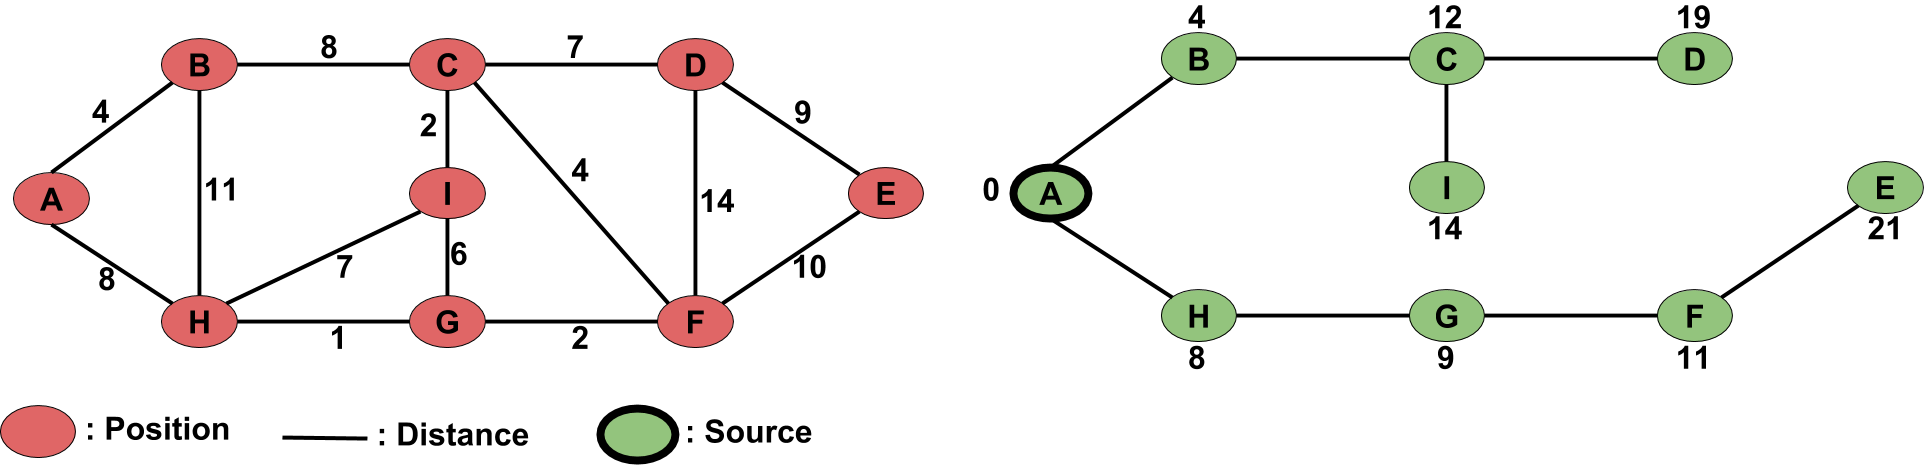
\includegraphics[width=160mm]{Figures/6.png}
\caption{Dijkstra pathfinding algorithm}
\end{center}
\end{figure*}
\vspace{-1cm}
\subsection{Detailed Routing}
The goal of detailed routing is to assign route segments of signal nets to specific routing tracks, vias, and metal layers with given global routes of those nets. For high performance analog circuits, constraints and objectives have to be considered. For the differential signal paths, the matching between parasitics on symmetrical nodes is often more important than their absolute values. For a given set of circuit specifications, several valid routing solutions can be found but with different yield, manufacturability and testability performances. Topology-matching and current-path constraints are commonly imposed on the critical, yet asymmetry nets with the same number of bends, vias, and wirelength to reduce current mismatches, sensitive nodes and noisy nodes that should not interact